%%%%%%%%%%%%%%%%%%%%%%%%%%%%%%%%%%%%%%%%%%%%%%%%%%%%%%%%%%%%%%%%%%%%%%%%%%%%%%%
%                          LaTeX beamer template                              %
%              © 2010 Valentin Roussellet (louen_AD_palouf.org)               %
%    Distributed under the terms of WTFPL v2, see http://sam.zoy.org/wtfpl    %
%%%%%%%%%%%%%%%%%%%%%%%%%%%%%%%%%%%%%%%%%%%%%%%%%%%%%%%%%%%%%%%%%%%%%%%%%%%%%%%
\documentclass{beamer}
% A reminder for beamer themes and colors
%                       Themes
% -----------------------------------------------------------------------------
% * Warsaw : black / colored toc above. Most commoly used
% * Copenhagen : like Warsaw without shadows
% * Marburg : black to blue right-sided toc
% * Berlin : colored panels above the text
% * Antibes : a lot like berlin
% * PaloAlto : colored left-sided toc
%                       Colors
%------------------------------------------------------------------------------
%   Name               background       titles          text
% * orchid (default)   white            dark blue       black
% * albatross          blue             light blue      white
% * beetle             grey             white           black
% * crane              white            black/yellow    black
% ============================== PREAMBLE =====================================
% Beamer settings ----------------
\mode<presentation>{
  %\usetheme{Marburg}                            % theme (see above)
  \usetheme{PaloAlto}                            % theme (see above)
  \usecolortheme{crane}                        % theme color (id)
  \setbeamercovered{transparent}                % For transparent zones
}

% Encoding and fonts -------------
\usepackage[utf8]{inputenc}                     % Input encoding
\usepackage[T1]{fontenc}                        % Output encoding
\usepackage{lmodern}                            % Modern font

% Language -----------------------
%\usepackage[right]{eurosym}                     % Symbol for euro

% Useful packages ----------------
\usepackage{listings}                           % for source code inclusion
\usepackage{hyperref}
% Mathematical symbols------------
\usepackage{amsmath}
\usepackage{amsfonts}
\usepackage{amssymb}

% Custom colors -----------------
\definecolor{codebg}{rgb}{0.97,0.97,0.97}
\definecolor{codecomment}{rgb}{0,0.5,0}
\definecolor{codestring}{rgb}{0.5,0,0}

% Listings setup -----------------
\lstset{language=C++,                             % programming language
%morekeywords={},                                % additionnal keywords
basicstyle=\small\ttfamily,                     % style of the code
keywordstyle=\color{blue}\bfseries,             % style of the keywords
stringstyle=\color{codestring},                 % style of the strings
commentstyle=\color{codecomment},               % style of the comments
showspaces=false,                               % do not underline spaces in code
showstringspaces=false,                         % do not underline spaces in strings
showtabs=false,                                 % do not underline tabs
numbers=left,                                   % where are the line-numbers
numberstyle=\tiny,                               % style of the line-numbers
backgroundcolor=\color{codebg},                 % background-color
stepnumber=1,                                   % the step between two line-numbers.
extendedchars=true,                             % allows extended characters
columns=flexible,                               % sets the columns to non-fixed width
tabsize=2,                                      % sets the tabulation width
frame=trBL,                                     % adds a frame around the code with double line on the bottom
frameround=tttt,                                % rounds the frame
breaklines=true,                                % line breaks automatically
breakautoindent=true,                           % keep indentation level withh line breaks
captionpos=b                                    % the caption is at the bottom
}

% Additional beamer commands ------
% this command prints a frame toc at each section beginning
\AtBeginSection[] {
  \begin{frame}
      \frametitle{What next ?}
      \tiny{\tableofcontents[currentsection]}
  \end{frame}
}

% ============================== FRONT MATTER =================================
\title{Magic : l'Assembleur}
\subtitle{Formation C++ bas niveau}
\author{Valentin \textsc{Roussellet}}
\institute[VIA]{Centrale Reseaux}
\date{\today}
\subject{}                                      % Information PDF
%\logo{\includegraphics[height=1cm]{logo.png}}  % Logo

% ============================= END OF PREAMBLE ===============================
\begin{document}
\begin{frame}
  \titlepage
\begin{center}
\href{mailto:louen@via.ecp.fr}{louen@via.ecp.fr}
\end{center}
\end{frame}
\section*{Introduction}
\begin{frame}
    \frametitle{Abandonnez tout espoir}
    \begin{center}
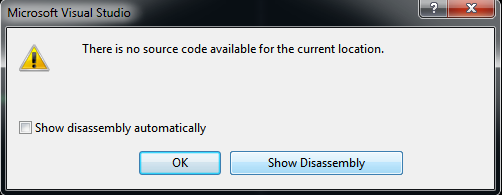
\includegraphics[scale=0.5]{disass.png}
\end{center}
\end{frame}

\begin{frame}
    \frametitle{Pourquoi connaitre l'assembleur}
Si vous vivez en 1895 (Nom de Zeus, Marty !)
\begin{itemize}
 \item Parce qu'il n'y a pas d'autre langage disponible
 \item Pour écrire du code super optimisé 
\end{itemize}
\pause
Mais en 2012 :
\begin{itemize}
 \item Pour comprendre ce qu'il se passe "sous le capot".
 \item Pour débugger quand on a pas la source (code optimisé par exemple)
\end{itemize}
\end{frame}

\begin{frame}
    \frametitle{Par ou commencer}
\begin{itemize}
 \item On va compiler du code C++ et regarder l'assembleur généré 
 \item J'utiliserai Visual Studio 2010 (syntaxe "Intel")
        \begin{itemize}
         \item Générer l'assembleur : \textbf{cl.exe /FA}
         \item Observer le code désassemblé : \textit{Debug > Windows > Disassembly}  
        \end{itemize}
        \pause
 \item Mais si vous êtes linuxien :
        \begin{itemize}
         \item Générer l'assembleur : \textbf{gcc -S}
         \item Observer le code désassemblé : \textbf{disass} dans gdb
         \item \textbf{-masm=intel} pour GCC ou \textbf{set disassembly-flavor intel} dans GDB pour avoir la syntaxe Intel  
        \end{itemize}
\pause
\item A la fin, vous en saurez un peu plus sur les \textbf{types}, les \textbf{pointeurs}, les \textbf{fonctions} et la \textbf{pile}, comment sont gérés les \textbf{objets} C++, et beaucoup d'autres choses.
\end{itemize}
\end{frame}
\begin{frame}
    \frametitle{Sommaire}
    \tiny{\tableofcontents}
\end{frame}

\section{Avengers, Disassemble !}
\begin{frame}[fragile]
  \frametitle{Notre premier désassemblage}

    \begin{lstlisting}
int x = 1;
int y = 2;
int z = 0;

z = x + y;
    \end{lstlisting}
\pause
    \begin{lstlisting}[language={[x86masm]Assembler}]
     ;1:         int x = 1;
00CB139E  mov         dword ptr [ebp-8],1  
     ;2:         int y = 2;
00CB13A5  mov         dword ptr [ebp-14h],2  
     ;3:         int z = 0;
00CB13AC  mov         dword ptr [ebp-20h],0  
     ;4: 
     ;5:         z = x + y;
00CB13B3  mov         eax,dword ptr [ebp-8]  
00CB13B6  add         eax,dword ptr [ebp-14h]  
00CB13B9  mov         dword ptr [ebp-20h],eax  
    \end{lstlisting}

\end{frame}
\begin{frame} [fragile]
\frametitle{Qu'est-ce que ca veut dire ?}
\begin{description}
\item[add] Instruction d'addition (you don't say ?)
\item[mov] Instruction qui copie de la mémoire : \lstinline[language={[x86masm]Assembler}]+mov dest src+
\item[eax] C'est un \textbf{registre} (mémoire embarquée du processeur). Les choses intéressantes se passent dans des registres.
\item[ebp] Un autre registre, appelé \textbf{base pointer}. On l'utilise pour accéder aux variables locales en mémoire.
\item[dword ptr] Valeur du mot mémoire de 32 bits situé a l'adresse entre crochets.
\end{description}
\end{frame}

\begin{frame} [fragile]
\frametitle{Qu'est-ce que ca veut dire ?}
    \begin{lstlisting}[language={[x86masm]Assembler}]
 ; la memoire a l'adresse ebp-8 (&x) prend la valeur 1
mov         dword ptr [ebp-8],1
 ; la memoire a ebp-14h (hex) prend la valeur 2.
mov         dword ptr [ebp-14h],2
 ; idem pour z. 
mov         dword ptr [ebp-20h],0
 ; charge le contendu de [ebp-8] (x) dans eax 
mov         eax,dword ptr [ebp-8]
 ; additione eax avec le contenu de [ebp-14h] (y)
add         eax,dword ptr [ebp-14h]
 ; deplace la valeur de eax dans [ebp-20h] (z)
mov         dword ptr [ebp-20h],eax
    \end{lstlisting}
\end{frame}

\begin{frame}
\frametitle{Pfiouu !}
\begin{itemize}
\item C'était pas si horrible !
\item En assembleur il y a les \textbf{instructions} (\lstinline[language={[x86masm]Assembler}]+mov+, \lstinline[language={[x86masm]Assembler}]+add+, etc.) et leurs \textbf{opérandes}.
\item Tout se passe avec les \textbf{registres} qui contiennent les résultats temporaires (\texttt{eax}, \texttt{ebx},...) ou servent a indexer la mémoire (\texttt{esp},\texttt{ebp}...).
\end{itemize}
\end{frame}

\section{Casse toi, pauvre type !}

\begin{frame}
\frametitle{Petit rappel sur les types} 

\begin{itemize}

\item En C : types \textit{fondamentaux} (mots-clefs du langage) 
\item 3 catégories : \textbf{void}, \textbf{entiers} et \textbf{nombres en virgule flottante}.
\item Chaque type a des \textit{specifications} déterminant leur représentation dans les types \textit{intrinseques} du CPU.
\pause 
\item Les types \textit{dérivés} : \textbf{pointeur} sur un type, \textbf{structure} ou \textbf{union} de plusieurs types.


\end{itemize}

\end{frame}

\begin{frame}
\frametitle{Les types entiers}
\begin{itemize}
\item Par ordre croissant de taille \lstinline+ char, short, int, long, long long+
\item Plus les variantes \lstinline+unsigned,  signed+ (quel est le défaut~?).
\item \lstinline+sizeof(char) == 1+ (et au moins 8 bits).
\item \lstinline+char*+ permet d'accéder a toute la mémoire.
\pause
\item Sur x86/Visual Studio 
\begin{description}
  \item[char] 1 octet ($-128$ a $127$ ou $0$ a $255$)
  \item[short] 2 octets ( $-32~768$ a $32~767$ ou $0$ a $65535$)
  \item[int] 4 octets ($-2~147~483~ 648$ a $2~147~483~ 647$ ou $0$ a $4~294~967~296$)
  \item[long] Identique a int.
  \item[long long] 8 octets (je vous laisse faire le calcul).
\end{description}

\end{itemize}
\end{frame}

\begin{frame}[fragile]
\frametitle{Types intrinseques}

\begin{itemize}
\item Les types réellement manipulés par le CPU : \textbf{intrinseques}
\item Sous x86 : \lstinline[language={[x86masm]Assembler}]+dword+ (32 bits) (\lstinline+word+ étant 16 bits)
\item Un type de 64 bits (\lstinline+long long+) sera représenté par deux \lstinline[language={[x86masm]Assembler}]+dword+s.
\end{itemize}

\begin{lstlisting}[language={[x86masm]Assembler}]
    ;10:   long long l = 1;
00E0139E  mov         dword ptr [ebp-0Ch],1  
00E013A5  mov         dword ptr [ebp-8],0  
    ;11:         long long m = 2;
00E013AC  mov         dword ptr [ebp-1Ch],2  
00E013B3  mov         dword ptr [ebp-18h],0  
    ;12:         long long n = l+m;
00E013BA  mov         eax,dword ptr [ebp-0Ch]  
00E013BD  add         eax,dword ptr [ebp-1Ch]  
00E013C0  mov         ecx,dword ptr [ebp-8]  
00E013C3  adc         ecx,dword ptr [ebp-18h]  
00E013C6  mov         dword ptr [ebp-2Ch],eax  
00E013C9  mov         dword ptr [ebp-28h],ecx 
\end{lstlisting}

\end{frame}

\begin{frame}
\frametitle{Représentation des entiers}
\begin{itemize}
\item \lstinline+unsigned+ : valeur binaire\\
exemple : \lstinline+unsigned short x = 0x8A2F+ = $35~375$

\item \lstinline+signed+ : \textbf{complément a deux} $ -i  = NOT(i) + 1 = 2^n - i $
 \begin{tabular}{c c c}
 127 & = & 0x7F\\
 ...& & \\
 2 & = & 0x02\\
 1 & = & 0x01\\
 0 & = & 0x00\\
-1 & = & 0xFF\\
-2 & = & 0xFE \\
...& &  \\
-127 & =&  0x81 \\
-128 & =&  0x80
\end{tabular}

\item Le type \lstinline +bool+ : pas de taille précisée, seulement 2 valeurs. (C++ seulement). 

\end{itemize}
\end{frame}

\begin{frame}
\frametitle{Représentation des réels}
\begin{itemize}
 \item Norme IEEE 754.
 \item \lstinline+float+ (4 octets), \lstinline+double+ (8 octets) \lstinline+long double+ (8 ou 10 octets)
\end{itemize}
\begin{tiny}
\begin{tabular} {|@{}c@{}|@{}c@{}|@{}c@{}|@{}c@{}|@{}c@{}|@{}c@{}|@{}c@{}|@{}c@{}|@{}c@{}|@{}c@{}|@{}c@{}|@{}c@{}|@{}c@{}|@{}c@{}|@{}c@{}|@{}c@{}|@{}c@{}|@{}c@{}|@{}c@{}|@{}c@{}|@{}c@{}|@{}c@{}|@{}c@{}|@{}c@{}|@{}c@{}|@{}c@{}|@{}c@{}|@{}c@{}|@{}c@{}|@{}c@{}|@{}c@{}|@{}c@{}|}
\hline

00&01&02&03&04&05&06&07&08&09&10&11&12&13&14&15&16&17&18&19&20&21&22&23&24&25&26&27&28&29&20&31\\
\hline
s & 
\multicolumn{8}{|c|}{exposant} & 
\multicolumn{23}{|c|}{mantisse} \\
\hline
\end{tabular}
\end{tiny}
\begin{itemize}
\item $val = s \times 2^{\mathrm{exposant}}\times \mathrm{mantisse}$
\item mantisse : chaque bit = $\frac{1}{2^b}$
\item Il y a donc $+0$ et $-0$
\item Ainsi que $+\infty$ et  $-\infty$
\item Des valeurs NaN et dénormalisées.
\item Attention a la précision (et a \lstinline+printf+)
\end{itemize}
\end{frame}


\begin{frame}
\frametitle{Les pointeurs}
\begin{itemize}
\item Les pointeurs \textbf{de données} ont tous la meme taille.
\item La taille des pointeurs définit l'\textit{espace adressable} 
\item Sur win32 : 32 bits (4Gib) -- mais ce n'est pas toujours la meme taille que \lstinline+int+ !
\end{itemize}

\end{frame}

\begin{frame}
\frametitle{Représentation mémoire : l'endianness}
\begin{itemize}
\item Ordre des octets : \textbf{big-endian} et \textbf{little-endian}  
\item Sur PC x86 (et x64) : c'est du little-endian.
\item D'autres machines sont big-endian : POWERPC (vieux Mac, XBox 360), Sun SPARC... 
\pause
\item On va regarder la mémoire pour voir comment est représenté un \lstinline+int+ 
\item Sous VS : \textit {Debug>Windows>Memory} (gdb : \textit{display})
\end{itemize}
\pause
\begin{itemize}
\item code : \lstinline+unsigned int x = 0x12345678;+
\item asm : \lstinline[language={[x86masm]Assembler}]+mov dword ptr [ebp-8],12345678h+
\item mémoire @ebp - 8 : \texttt{0x004BF848  78 56 34 12}
\end{itemize}

% parallele avec les dates.


\end{frame}
\begin{frame}[fragile]
\frametitle{Alignement et remplissage}
\begin{itemize}
\item Les données sont alignées sur la taille d'un mot.
\end{itemize}
\begin{columns}
  \begin{column}{0.3\textwidth}
\begin{lstlisting}

struct Test {
  int a;
  char b;
  long c;
};
\end{lstlisting}
  \end{column}
  \begin{column}{0.5\textwidth}
\begin{lstlisting}
int main() {
  struct Test inst;
  inst.a = 42;
  inst.b = '@';
  inst.c = 0x12345678;
}
\end{lstlisting}
  \end{column}
\end{columns}
\pause
\begin{itemize}
\item Résultat dans la mémoire : 
\end{itemize}
\begin{lstlisting}
0x003EF8FC  2a 00 00 00  // a (32 b)  
0x003EF900  40 cc cc cc  // b (8 b) + 24 b de 'padding' 
0x003EF904  78 56 34 12  // c (32b) 
\end{lstlisting}

\end{frame}

\begin{frame}[fragile]
\frametitle{Alignement et remplissage}
\begin{itemize}
\item On peut changer le comportement du compilateur 
\end{itemize}
\begin{columns}
  \begin{column}{0.3\textwidth}
\begin{lstlisting}
#pragma pack(1)
struct Test {
  int a;
  char b;
  long c;
};
\end{lstlisting}
  \end{column}
  \begin{column}{0.5\textwidth}
\begin{lstlisting}
int main() {
  struct Test inst;
  inst.a = 42;
  inst.b = '@';
  inst.c = 0x12345678;
}
\end{lstlisting}
  \end{column}
\end{columns}
\pause
\begin{itemize}
\item Résultat dans la mémoire : 
\end{itemize}
\begin{lstlisting}
0x003EF8FC  2a 00 00 00  // a (32 b)  
0x003EF904  40 78 56 34  // b (8b) + 24 premiers b de c 
0x003EF900  12 cc cc cc  // fin de c 
\end{lstlisting}
\end{frame}
\begin{frame}
\frametitle{Alignement et remplissage}
\begin{itemize}
\item Sous x86 on peut accéder aux données meme non-alignées
\item ...sauf dans certains cas (SIMD par exemples).
\item Le compilateur aligne par défaut et remplit les structures avec du vide
\item ... mais on peut le contraindre : attention a la portabilité !
\end{itemize}
\end{frame}

\begin{frame}
\frametitle{Ouf !}
On a vu pas mal de parametres a prendre en compte pour les types et leur représentation
\begin{itemize}
\item Leur taille (par rapport au types intrinseques)
\item La convention de signe (ou pas).
\item La représentation des flottants (exposant et mantisse)
\item L'endianness
\item L'alignement
\end{itemize}
\end{frame}

\section{Sexe a Pile}

\begin{frame}
\frametitle{A la recherche de La Pile}
Ce que vous devriez savoir de La Pile (\textit{stack}).
\begin{itemize}
\item C'est une pile (surprise !)
        \begin{itemize}
        \item Il y a donc les opérations \texttt{push()}, \texttt{pop()} et  \texttt{top()}
        \end{itemize}
\item Elle contient les variables \textbf{automatiques} 
\item C'est la que sont passés les \textbf{arguments} des fonctions (\textit{stack frame})
\end{itemize}
\end{frame}


\begin{frame}
\frametitle{Stack frame et appel de fonction}
Que se passe t'il quand on appelle une fonction ?
\begin{itemize}
\item L'état courant du processeur (i.e. les valeurs des registres) est sauvé sur la Pile.
\item Les arguments de la fonction appelée sont positionnés sur la Pile
\item L'ensemble de ces données : le \textbf{stack frame}.
\item Le CPU "saute" a l'adresse de la fonction appelée.
\end{itemize}
Si on break, on peut voir les stack frames des fonctions empilés :
\begin{itemize}
\item Valeur des parametres et variables locales
\item Contenu des registres utilisés au moment ou l'appel suivant a été fait
\item Adresse de retour de la fonction apres \lstinline+return+
\end{itemize} 
\end{frame}

\begin{frame}
\frametitle{Les conventions d'appel} % mettr ça plus haut ?
La convention d'appel standard de VS/x86 s'appelle \texttt{stdcall}
\begin{itemize}
\item Ou vont les paramètres ? Sur la pile !
\item Ou est la valeur de retour ? dans \texttt{eax}
\item Qui vide la pile après l'appel ? l'appelé.
\item Qui sauve quels registres ? l'appelant (\texttt{eax}-\texttt{edx}) et l'appelé le reste
\end{itemize}
\end{frame}
% TODO  : image d'un stack frame ?

\begin{frame}[fragile]
\frametitle{Désassemblons !}
Un petit code tout innoffensif :
\begin{lstlisting}
int ajouterUn( int argument ){
  int local = argument + 1;
  return local;
}

int main() {
  int result = 0;
  result = ajouterUn(result);
  return 0;
}
\end{lstlisting}
\begin{itemize}
\item On met un point d'arret ligne 6 (\lstinline+int main()+)...
\end{itemize}
\end{frame}

\begin{frame}[fragile]
\frametitle{Désassemblons !}
\begin{lstlisting}[language={[x86masm]Assembler}, basicstyle={\scriptsize\ttfamily}]
push        ebp  
mov         ebp,esp  
sub         esp,44h  
push        ebx  
push        esi  
push        edi  
;     7:         int result = 0;
mov         dword ptr [ebp-4],0  
;     8:         result = ajouterUn(result);
mov         eax,dword ptr [ebp-4]  
push        eax  
call        00C81041  
add         esp,4  
mov         dword ptr [ebp-4],eax  
;     9:         return 0;
xor         eax,eax  
    10: }
pop         edi  
pop         esi  
pop         ebx  
mov         esp,ebp  
pop         ebp  
ret  
\end{lstlisting}
\end{frame}
\begin{frame}[fragile]
\frametitle{Don't panic !}
\begin{description}
\item[esp]  \textbf{Stack Pointer} : pointe en "haut" de la Pile 
\item[ebp]  \textbf{Base Pointer} : pointe au début du stack frame courant.
\end{description}
\begin{itemize}
\item Les variables sur la Pile sont référencées par rapport a \texttt{ebp} : \lstinline[language={[x86masm]Assembler}]+dword ptr [ebp-4]+ 
\item Mais alors pourquoi des soustractions ?
\pause
\item Parce que la pile grandit vers le bas ! (le "haut" a une adresse plus petite que le "bas").
\end{itemize}
\end{frame}

\begin{frame}[fragile]
\frametitle{Push it, pop it}
\begin{itemize}
\item Quand on \texttt{push} : \texttt{esp} est décrémenté, et l'opérande est stocké dans l'espace pointé par \texttt{esp}
\item \texttt{esp} pointe donc sur la derniere valeur ajoutée dans la stack
\item Quand on pop, l'a mémoire par \texttt{esp} est copiée dans un registre et \texttt{esp} est incrémenté (la pile diminue)
\end{itemize}
\pause
En résumé :
\begin{itemize}
\item  \lstinline[language={[x86masm]Assembler}]+push ecx+ $\rightarrow$ \lstinline+esp --; *esp = ecx;+ 
\item  \lstinline[language={[x86masm]Assembler}]+pop ebx+ $\rightarrow$  \lstinline!ebx = *esp; esp++;!
\end{itemize}
\end{frame}



\begin{frame}[fragile]
\frametitle{Le préambule} 
\begin{lstlisting}[language={[x86masm]Assembler}, basicstyle={\scriptsize\ttfamily}]
push        ebp ; l'ancien bp est sauve
mov         ebp,esp  ; nouveau bp
sub         esp,44h  ; ajoute de l'espace
push        ebx  ; sauve les registres
push        esi  
push        edi  
\end{lstlisting}
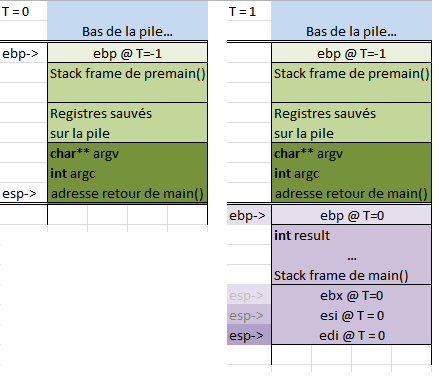
\includegraphics[scale=0.5]{stack_01.png}
\end{frame}

% image avant -> après 
\begin{frame}[fragile]
\frametitle{L'épilogue}
Il fait l'inverse du préambule :
\begin{lstlisting}[language={[x86masm]Assembler}, basicstyle={\scriptsize\ttfamily}]
013112A1  pop         edi
013112A2  pop         esi
013112A3  pop         ebx
013112A4  mov         esp,ebp ; restore esp a son ancienne valeur
013112A6  pop         ebp ; l'ancien bp est juste la !
013112A7  ret
\end{lstlisting}
\includegraphics[scale=0.5]{stack_1.png}
\end{frame}

\begin{frame}[fragile]
\frametitle{Et notre code ?}
\begin{lstlisting}[language={[x86masm]Assembler}, basicstyle={\scriptsize\ttfamily}]
;     7: int result = 0;
mov         dword ptr [ebp-4],0  ; result est a ebp-4 dans notre SF 
;     8: result = ajouterUn(result);
mov         eax,dword ptr [ebp-4] ; copie le parametre  (via eax)
push        eax                   ; pour le mettre sur la pile 
call        00C81041              ; saute a l'adresse de la fonction
add         esp,4                 ; pareil que pop(ignore la valeur)
mov         dword ptr [ebp-4],eax ; le resultat (eax) va dans result
;     9:         return 0;
xor         eax,eax  
\end{lstlisting}
\begin{itemize}
\item Le parametre est copié sur la pile (via un registre)
\item On sait que le résultat est dans \texttt{eax}.
\end{itemize}
\end{frame}

\begin{frame}[fragile]
\frametitle{Notre fonction}
Il est temps (enfin) de désassembler notre fonction !
\begin{lstlisting}[language={[x86masm]Assembler}, basicstyle={\scriptsize\ttfamily}]
; 1: int ajouterUn( int argument ){
push        ebp      ;preambule : on connait !
mov         ebp,esp  
sub         esp,44h  
push        ebx  
push        esi  
push        edi  
;2: 	int local = argument + 1;
mov         eax,dword ptr [ebp+8]  ;c'est hors de notre SF
add         eax,1  
mov         dword ptr [ebp-4],eax  ; variable locale dans notre SF
;3: 	return local;
mov         eax,dword ptr [ebp-4]  ; resultat dans eax
;4: }
pop         edi  ; epilogue : on connait aussi
pop         esi  
pop         ebx  
mov         esp,ebp  
pop         ebp  
ret  
\end{lstlisting}

\end{frame}

\begin{frame}[fragile]
\frametitle{Notre fonction}

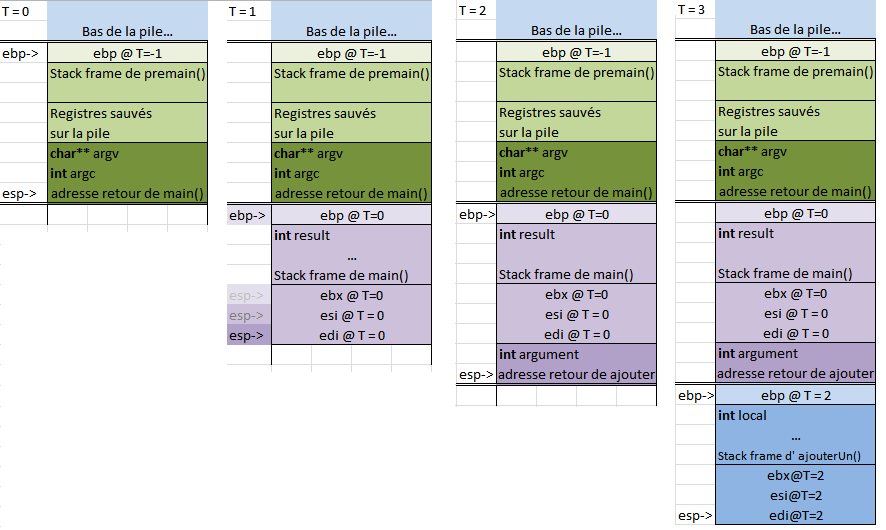
\includegraphics[scale=0.45]{stack.png}
\end{frame}

\begin{frame}[fragile]
\frametitle{Résumé}
La pile sert a :
\begin{itemize}
\item Stocker les variables locales
\item Sauver les registres et passer les parametres (un ou plusieurs !)
\end{itemize}
La \textbf{convention d'appel} détermine qui fait quoi sur la pile.

Le \textbf{stack frame}
\begin{itemize}
\item Un par appel de fonction
\item Compris entre \texttt{esp} et \texttt{ebp}
\item Les arguments : dans le SF de la fonction appelante
\end{itemize}

\end{frame}

\section{Condition zéro}
\begin{frame}[fragile]
\frametitle{If I had a hammer}
\begin{itemize}
\item Démarrons avec un code tres facile :
\end{itemize}
\begin{lstlisting}
int f (int arg) {
  int local = 0;
  if ( arg < 0 ) {
    local = 1;
  }
  return 0;
}
\end{lstlisting}
\end{frame}

\begin{frame}[fragile]
\frametitle{If I had a hammer}
\begin{itemize}
\item Voila ce que donne le désassemblage : 
\end{itemize}
\begin{lstlisting}[language={[x86masm]Assembler}]
;2:         int local = 0;
00B91299  mov         dword ptr [ebp-4],0  
;3:         if ( arg < 0 ) {
00B912A0  cmp         dword ptr [ebp+8],0  
00B912A4  jge         00B912AD  
;4:                 local = 1;
00B912A6  mov         dword ptr [ebp-4],1  
;5:         }
;6:         return 0;
00B912AD  xor         eax,eax  
\end{lstlisting}
\end{frame}

\begin{frame}[fragile]
\frametitle{Que remarquons-nous ?}
\begin{itemize}
\item La ligne du \lstinline+if+ devient deux instructions
\begin{description} 
\item[cmp] comparaison (aucun effet mais change les EFLAGS)
\item[jge] Jump if Greater or Equal  : saute a l'adresse indiquée selon la valeur des EFLAGS
\end{description} 
\pause
\item C'est l'inverse de ce qu'on a écrit en C !
\pause
\item \textbf{si} \textit{condition} \textbf{alors} entrer dans les accolades
\item \textbf{si} $\neg$\textit{condition} \textbf{alors} sauter 
\end{itemize}


\begin{lstlisting}
int local = 0;
if ( arg >= 0 ) goto Positive;
local = 1;
Positive:
return 0;
\end{lstlisting}
\pause
\begin{itemize}
\item Bonus : c'est le registre \textbf{eip} (instruction pointer) qui est modifié par \texttt{jge} !)
\end{itemize}
\end{frame}

\begin{frame}[fragile]
\frametitle{Un peu plus complexe}
\begin{lstlisting}
int local = 0;
if ( arg == 0 ){
  local = 12;
}
else if (arg != 42) {
  local = 6 * 9;
}
else {
	local = 666;
}
return 0;
\end{lstlisting}
\end{frame}

\begin{frame}[fragile]
\frametitle{Un peu plus complexe}
\begin{lstlisting}[language={[x86masm]Assembler}, basicstyle={\scriptsize\ttfamily}]
;     2: 	if ( arg == 0 ){
00F51260  cmp         dword ptr [ebp+8],0  
00F51264  jne         0F5126Fh ; jump if not equal 
;     3: 	  local = 12;
00F51266  mov         dword ptr [ebp-4],0Ch  
00F5126D  jmp         0F51285h; on sort du bloc if 
;     4: 	}
;     5: 	else if (arg != 42) {
00F5126F  cmp         dword ptr [ebp+8],2Ah  
00F51273  je          0F5127Eh  ; jump if equal
;     6: 	  local = 6 * 9;
00F51275  mov         dword ptr [ebp-4],36h  
00F5127C  jmp         0F51285h   ; on sort du bloc if
;     7: 	}
;     8: 	else {
;     9: 	  local = 666;
00F5127E  mov         dword ptr [ebp-4],29Ah ; 
;    10: 	}
;    11: 	return 0;
00F51285  xor         eax,eax  
\end{lstlisting}
\end{frame}

\begin{frame}[fragile]
\frametitle{Dernier exemple : opérations logiques}
\begin{lstlisting}
int f (int arg) {
  int local = 0;

  if ( arg >= 7 && arg <= 12){
    local = 9001;
  }
  else if (arg || ! arg || arg == 69 ) { // stupide :)
    local = 6 * 9;
  }
  return 0;
}
\end{lstlisting}
\end{frame}

\begin{frame}[fragile]
\frametitle{Dernier exemple : operations logiques}
\begin{lstlisting}[language={[x86masm]Assembler}, basicstyle={\scriptsize\ttfamily}]
;    4: 	if ( arg >= 7 && arg <= 12){
00E61260  cmp         dword ptr [ebp+8],7  ; condition 1
00E61264  jl          00E61275             ; saute au else si arg < 7
00E61266  cmp         dword ptr [ebp+8],0Ch  ; condition 2 
00E6126A  jg          00E61275               ; saute au else si arg > 12
;     5: 	  local = 9001;
00E6126C  mov         dword ptr [ebp-4],2329h  
00E61273  jmp         00E6128E  
;     6: 	}
;     7: 	else if (arg || ! arg || arg == 69 ) {
00E61275  cmp         dword ptr [ebp+8],0 condition 1 
00E61279  jne         00E61287            ; surprise ! pas d'inversion
00E6127B  cmp         dword ptr [ebp+8],0  
00E6127F  je          00E61287            ; toujours pas d'inversion
00E61281  cmp         dword ptr [ebp+8],45h  
00E61285  jne         00E6128E            ; cette fois si.
;     8: 	  local = 6 * 9;
00E61287  mov         dword ptr [ebp-4],36h  
;     9: 	}
;    10: 	return 0;
00E6128E  xor         eax,eax  
;    11: }
\end{lstlisting}
\end{frame}

\begin{frame}
\frametitle{Résumons}
\begin{itemize}
\item Chaque condition est transformée en \texttt{cmp} et \texttt{jXX}
\item Les conditions des sauts conditionnels sont \textbf{inversées} par rapport au \texttt{if}.
\item L'évaluation "paresseuse" des conditions se fait naturellement : chaque "atome" génere un couple comparaison + saut.
\item Testez avec un operateur ternaire (\texttt{ a?b:c;}) ou un \lstinline+switch+.
\end{itemize}
\end{frame}



\section{La boucle est bouclée}
\begin{frame}[fragile]
\frametitle{Petite histoire des boucles}
Protozoaire supérieur : \lstinline+if+ - \lstinline+goto+
\begin{lstlisting}
int main() {
  int tab [5] ={ 8, 4, 22, 904, 30 };
  int somme = 0;  int compteur = 0;

DebutBoucle:
  if (compteur < 5 ){
    somme += tab[compteur];
    ++compteur;
    goto DebutBoucle;
  }
  return 0;
}
\end{lstlisting}
\end{frame}

\begin{frame}[fragile]
\frametitle{Étudions ce fossile}
\begin{lstlisting}[language={[x86masm]Assembler}, basicstyle={\scriptsize\ttfamily}]
;     5: DebutBoucle:
;     6: 	if (compteur < 5 ) {
013F1284  cmp         dword ptr [ebp-20h],5 ; on reconnait un if
013F1288  jge         13F12A2h              ; cmp + jump !
;     7: 		somme += tab[compteur];
013F128A  mov         eax,dword ptr [ebp-20h]       ; compteur dans eax
013F128D  mov         ecx,dword ptr [ebp-1Ch]       ; somme dans ecx
013F1290  add         ecx,dword ptr [ebp+eax*4-18h] ; WTF ?? 
013F1294  mov         dword ptr [ebp-1Ch],ecx       ; resultat dans somme
;     8: 		++compteur;
013F1297  mov         eax,dword ptr [ebp-20h]  
013F129A  add         eax,1  
013F129D  mov         dword ptr [ebp-20h],eax  
;     9: 		goto DebutBoucle;
013F12A0  jmp         13F1284h  
;    10: 	}
;    11: 	return 0;
013F12A2  xor         eax,eax  
\end{lstlisting}
\end{frame}

\begin{frame}[fragile]
\frametitle{Tombés sur un os}
\begin{itemize}
\item  \lstinline[language={[x86masm]Assembler}]@add ecx,dword ptr [ebp+eax*4-18h]@
\item On veut accéder a l'élément du tableau désigné par \texttt{compteur} (dans \texttt{eax}).
\item Réarangeons la formule : \texttt{(epb - 18h) + (eax * 4)}
\item \lstinline@ &tab[0] + (compteur * sizeof(int))@
\end{itemize}
\end{frame}

\begin{frame}[fragile]
\frametitle{Petite histoire des boucles}
Bas Moyen-Age : \lstinline+while+
\begin{lstlisting}
int main() {
  int tab [5] ={ 8, 4, 22, 904, 30 };
  int somme = 0;  int compteur = 0;
  
  while (compteur < 5 ){
    somme += tab[compteur];
    ++compteur;
  }
  return 0;
}
\end{lstlisting}
\end{frame}

\begin{frame}[fragile]
\frametitle{Faith in humanity restored}
\begin{lstlisting}[language={[x86masm]Assembler}, basicstyle={\scriptsize\ttfamily}]
;     5:  while (compteur < 5 ){
01161284  cmp         dword ptr [ebp-20h],5  
01161288  jge         11612A2h  
;     6: 		somme += tab[compteur];
0116128A  mov         eax,dword ptr [ebp-20h]  
0116128D  mov         ecx,dword ptr [ebp-1Ch]  
01161290  add         ecx,dword ptr [ebp+eax*4-18h]  
01161294  mov         dword ptr [ebp-1Ch],ecx  
;     7: 		++compteur;
01161297  mov         eax,dword ptr [ebp-20h]  
0116129A  add         eax,1  
0116129D  mov         dword ptr [ebp-20h],eax  
;     8: 	}
011612A0  jmp         1161284h  
;     9: 	return 0;
011612A2  xor         eax,eax  
\end{lstlisting}
Vous pouvez vérifier le \lstinline+do{...} while(...)+.
\end{frame}

\begin{frame}[fragile]
\frametitle{Petite histoire des boucles}
Époque moderne : \lstinline+for+
\begin{lstlisting}
int main() {
  int tab [5] ={ 8, 4, 22, 904, 30 };
  int somme = 0;  
  for (int compteur = 0; compteur < 5; ++compteur){
    somme += tab[compteur];
  }
  return 0;
}
\end{lstlisting}
\end{frame}

\begin{frame}[fragile]
\frametitle{Hail to the king, baby!}
\begin{lstlisting}[language={[x86masm]Assembler}, basicstyle={\scriptsize\ttfamily}]
;     5: 	for (int compteur = 0; compteur < 5; ++compteur){
00AA127D  mov         dword ptr [ebp-20h],0    ; compteur = 0
00AA1284  jmp         00AA128F  

00AA1286  mov         eax,dword ptr [ebp-20h]  
00AA1289  add         eax,1                    ; ++compteur
00AA128C  mov         dword ptr [ebp-20h],eax  

00AA128F  cmp         dword ptr [ebp-20h],5  ;on retrouve notre if 
00AA1293  jge         00AA12A4               ;(test de sortie de boucle)

;     6: 		somme += tab[compteur];
00AA1295  mov         eax,dword ptr [ebp-20h]  
00AA1298  mov         ecx,dword ptr [ebp-1Ch]  
00AA129B  add         ecx,dword ptr [ebp+eax*4-18h]  
00AA129F  mov         dword ptr [ebp-1Ch],ecx  
;     7: 	}
00AA12A2  jmp         00AA1286  
;     8: 	return 0;
00AA12A4  xor         eax,eax  
;     9: }
\end{lstlisting}
\end{frame}

\begin{frame}[fragile]
\frametitle{Final : hardcore loop porn}
Etes vous prets a affronter de l'assembleur optimisé ?
\begin{lstlisting}
#include <cstdlib>
int main(int argc, char**argv) {
  int tab [5] ={ 8, 4, 22, 904, 30 };
  int somme = 0;	
  int taille = atoi(argv[0]);
  for (int compteur = 0; compteur<taille; ++compteur){
    somme += tab[compteur];
  }
  return 0;
}
\end{lstlisting}
\begin{itemize}
\item \textbf{/O2} : Active les optimisations
\item \textbf{/Ob0} : Désactive l'inlining
\end{itemize}
\end{frame}

\begin{frame}[fragile]
\frametitle{Hardcore loop porn}
\begin{lstlisting}[language={[x86masm]Assembler}, basicstyle={\scriptsize\ttfamily}]
00F21042  xor       ecx,ecx   ; ecx = 0 
00F21044  cmp       eax,2     ; si eax est < 2
00F21047  jl        0F2105Fh  ; sauter a la fin de la boucle 
00F21049  lea       edx,[eax-1]  ; edx = eax -1
00F2104C  lea       esp,[esp]  
; -- debut  boucle
00F21050  add       esi,dword ptr [ebp+ecx*4-14h]; esi += tab [i] 
00F21054  add       edi,dword ptr [ebp+ecx*4-10h]; esi += tab [i + 1]
00F21058  add       ecx,2;		  ecx = ecx + 2
00F2105B  cmp       ecx,edx   ; si ecx est < eax -1 
00F2105D  jl        0F21050h  ; boucler
; -- fin boucle
00F2105F  cmp       ecx,eax   ; si ecx est < eax 
00F21061  jge       0F21067h  ; sauter l'instruction suivante (pair)
00F21063  mov       ebx,dword ptr ebx,dword ptr [ebp+ecx*4-14h]   
00F21067  lea       eax,[edi+esi]  ; eax = somme finale
00F2106A  pop       edi  
00F2106B  pop       esi  
00F2106C  add       eax,ebx  ; eax += impair eventuel
\end{lstlisting}
\end{frame}

\begin{frame}[fragile]
\frametitle{Final : hardcore loop porn}
\begin{itemize}
\item Au niveau de l'assembleur les boucles ne sont pas si différentes du  \lstinline+if+ - \lstinline+goto+.
\item Mais elles automatisent les choses (et évitent de se tromper)
\item Nous avons vu un exemple d'optimisation : le déroulage de boucle
\end{itemize}
\end{frame}

\begin{frame}[fragile]
\frametitle{Fini !}

\begin{itemize}
\item Alex Darby, \textit{A Low Level Curriculum For C and C++} (\href{http://http://www.altdevblogaday.com/2011/11/09/a-low-level-curriculum-for-c-and-c/}{AltDevBlogADay})
\item \textit{Intel IA 32 Architecture Software Developper Manual} (\href{http://download.intel.com/products/processor/manual/325462.pdf}{intel.com})
\item MazeGen, \textit{coder32} ASM reference (\href{http://ref.x86asm.net}{refx86asm.net})
\end{itemize}

\begin{center}
\begin{large}
\lstinline[language={[x86masm]Assembler}]+ret+ 
\end{large}
\end{center}
\end{frame}

%  \begin{block}{A block}
%   Text in a block
%  \end{block}
%  \begin{exampleblock}{Another block}
%   Text in an example block
%  \end{exampleblock}
%  \pause
%  \begin{alertblock}{Yet another block}
%   Text in an warning block
%  \end{alertblock}

% WARNING : every frame with code in it must be declared [fragile]
% and the \end{frame} should not be indented (see beamer documentation)
\end{document}
